\section{Toward an eclectic and malleable multiagent educational assistant \cite{briel2021}}
\label{sec:briel2021}

%Agentes conversacionais são sistemas capazes de processar e responder linguagem natural. Eles evoluíram com o passar dos anos, indo desde um meio para passar no Teste de Turing até chatbots que possuem um objetivo utilitário, como suporte ao cliente \apud{briel2021}{cui2017} e tutoria \apud{briel2021}{wang2013}. Uma distinção pode ser feita entre agentes de domínio aberto e domínio fechado, enquanto os de domínio aberto são capazes de manter uma conversa sobre diversos assuntos, os de domínio fechado são mais orientadas à tarefas e tendem a conseguir retornar informações para uma variedade de solicitações.

Chatbots de domínio fechado são frequentemente limitados em funcionalidade, seja por serem capazes de conversar sobre apenas um domínio específico, responder apenas à perguntas simples ou buscar arquivos. Apesar dessas limitações, existe uma ampla variedade de funcionalidades possíveis que um agente pode oferecer, podendo até ser um assistente educacional e fornecer recomendações de materiais acadêmicos.

Um sistema que é capaz de executar todas essas funcionalidades acima simultaneamente se destacaria dos demais agentes que possuem apenas uma única função. Com base nas necessidades dos alunos, funções diferentes, como fornecer links, resumos ou conteúdos abrangendo várias bases de conhecimento, podem facilitar o aprendizado individual. Assim, para atender a essas necessidades, no artigo de \citeonline{briel2021}, é proposto um framework multiagente chamado JuggleChat, formado internamento por vários chatbots e outros componentes relacionados, que possui foco na diversidade de funções do chatbot e não apenas no conhecimento de domínio fechado.

Conforme descrito na Figura \ref{fig:architecture-briel}, a arquitetura do JuggleChat é constituída por uma interface do usuário, um módulo de extração da intenção da mensagem, um alocador de chatbots e vários chatbots internos. Com isso, no fluxo de dados, a entrada do usuário é processada pelo módulo de extração da intenção. Em seguida, a intenção e a entrada são passadas para o alocador de chatbots que, com base na intenção, define para qual chatbot interno será direcionada a mensagem. Por fim, o respectivo chatbot processa a mensagem e gera uma resposta, que é então enviada para o usuário.

\begin{figure}[ht] 
   	\captionsetup{width=16cm}
	\Caption{\label{fig:architecture-briel} Arquitetura do JuggleChat}
	\UFCfig{}{
        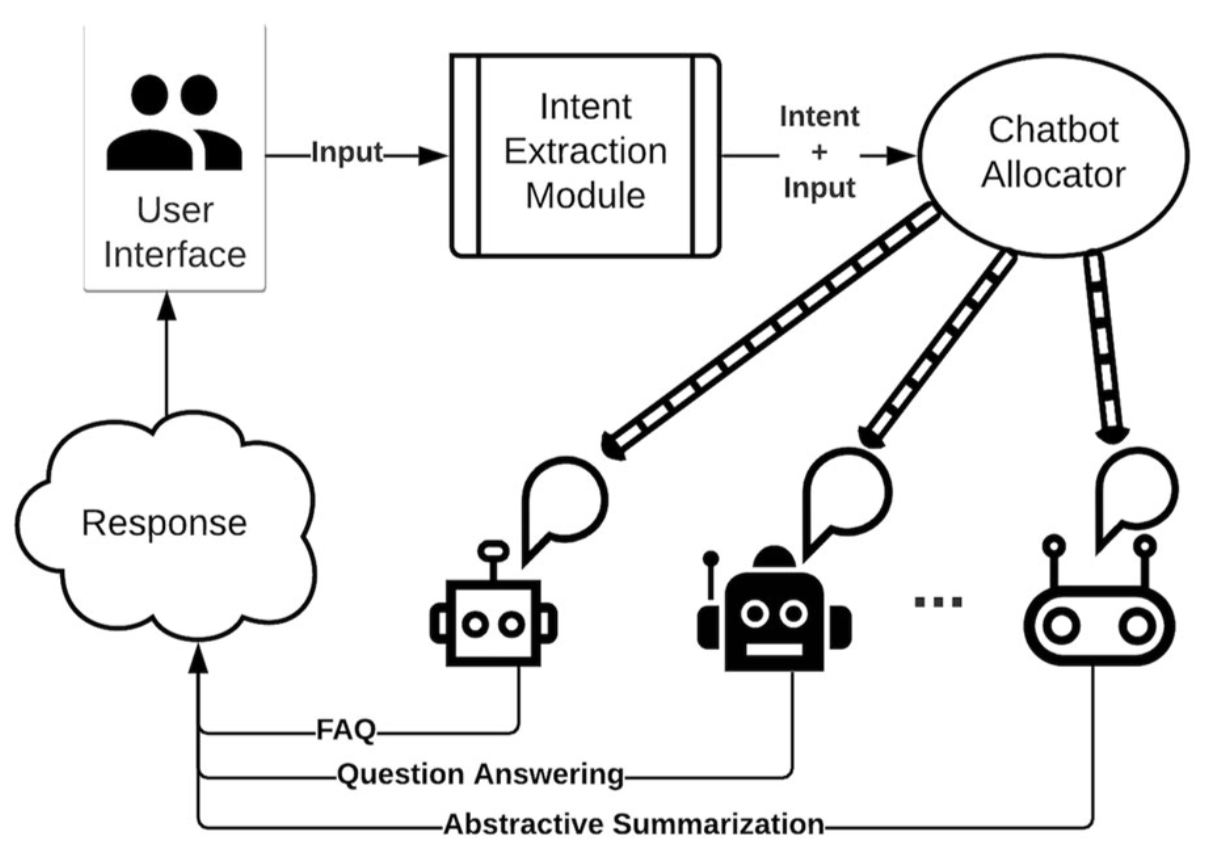
\includegraphics[width=16cm]{figuras/architecture-briel.png}
    }{
		\Fonte{\citeonline{briel2021}.}
	}
\end{figure}

A arquitetura desse estudo foi planejada usando bibliotecas e componentes de código aberto. A interface do usuário para o processamento de entradas e entrega de respostas foi construída usando React e TypeScript, com seu backend constituído por um servidor Express que se comunica com um banco de dados PostgreSQL. Uma instância do Rasa foi utilizada para o módulo de extração da intenção do usuário.

Os dois principais objetivos do experimento foram determinar a eficiência do JuggleChat como ferramenta de auxílio aos estudantes durante o aprendizado, e entender como os participantes se sentem durante a interação com o chatbot e como eles percebem sua precisão e utilidade.

Quatro grupos de cem participantes cada foram usados para avaliar o uso do framework, e ninguém sabia da tecnologia subjacente do chatbot que estavam usando. O primeiro grupo usou apenas um chatbot baseado em respostas curtas. Já o segundo grupo usou apenas um chatbot baseado em respostas longas. O terceiro grupo usou o JuggleChat que continha os dois chatbots citados anteriormente, além de possuir um módulo de sumarização e a capacidade de enviar URLs. O quarto grupo não fez uso de chatbots. Os grupos que possuíam acesso ao chatbot foram alocados para avaliar o sistema multiagente no geral e os chatbots usados internamente, já o objetivo de ter um grupo que não fazia de uso de chatbots foi para mensurar o quanto o acesso aos chatbots afetaria a performance do teste.

Em um primeiro momento, foi passado para os participantes um conjunto de instruções indicando que eles teriam uma lição sobre informações relacionadas ao COVID-19. Caso eles fizessem parte de um dos três grupos que usariam o chatbot, também foi repassado que eles poderiam fazer cinco perguntas para um chatbot (Figura \ref{fig:conversation-briel}), depois avaliar a interação com ele (Figura \ref{fig:evaluation-briel}), e no final, realizar um questionário sobre o conteúdo (Figura \ref{fig:quiz-briel}). Os participantes que não usariam o chatbot apenas receberam a instrução que eles realizariam um questionário após o término da lição (Figura \ref{fig:quiz-briel}).

\begin{figure}[ht] 
   	\captionsetup{width=16cm}
	\Caption{\label{fig:conversation-briel} Exemplo de interação com o JuggleChat}
	\UFCfig{}{
        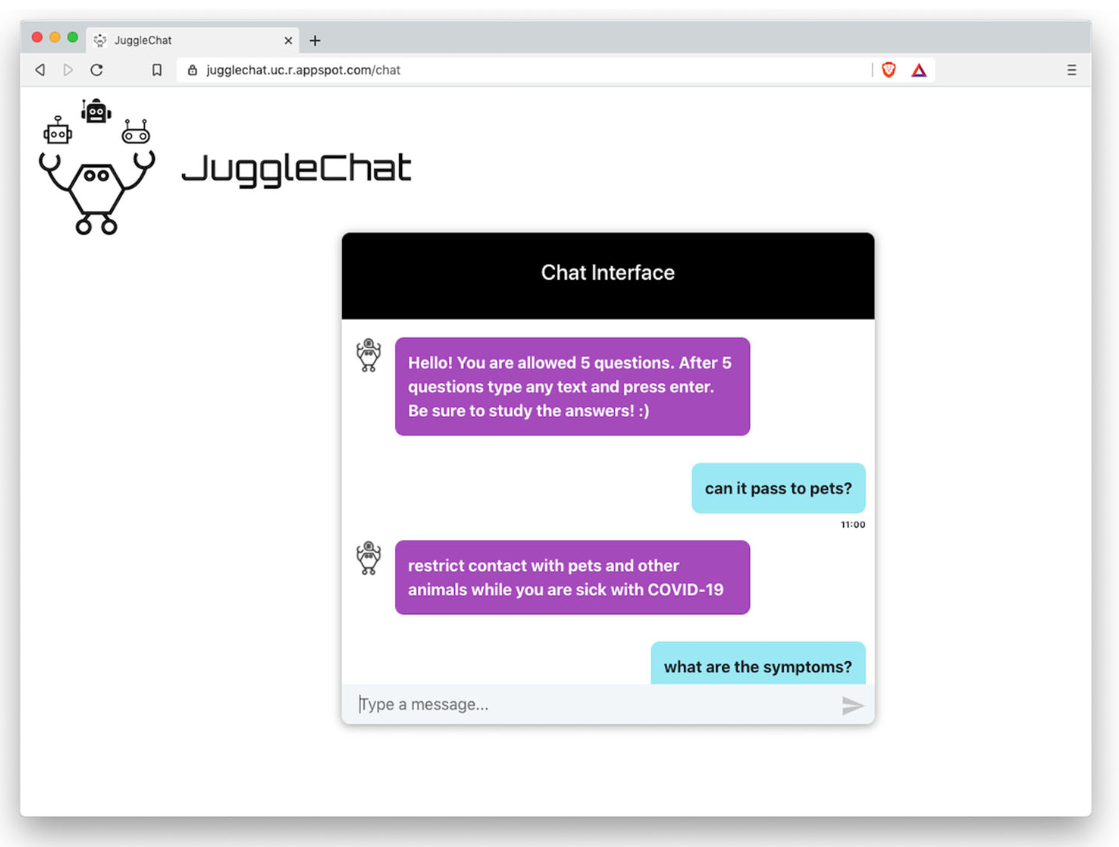
\includegraphics[width=16cm]{figuras/conversation-briel.png}
    }{
		\Fonte{\citeonline{briel2021}.}
	}
\end{figure}

\begin{figure}[ht] 
   	\captionsetup{width=16cm}
	\Caption{\label{fig:evaluation-briel} Avaliação da interação com o JuggleChat}
	\UFCfig{}{
        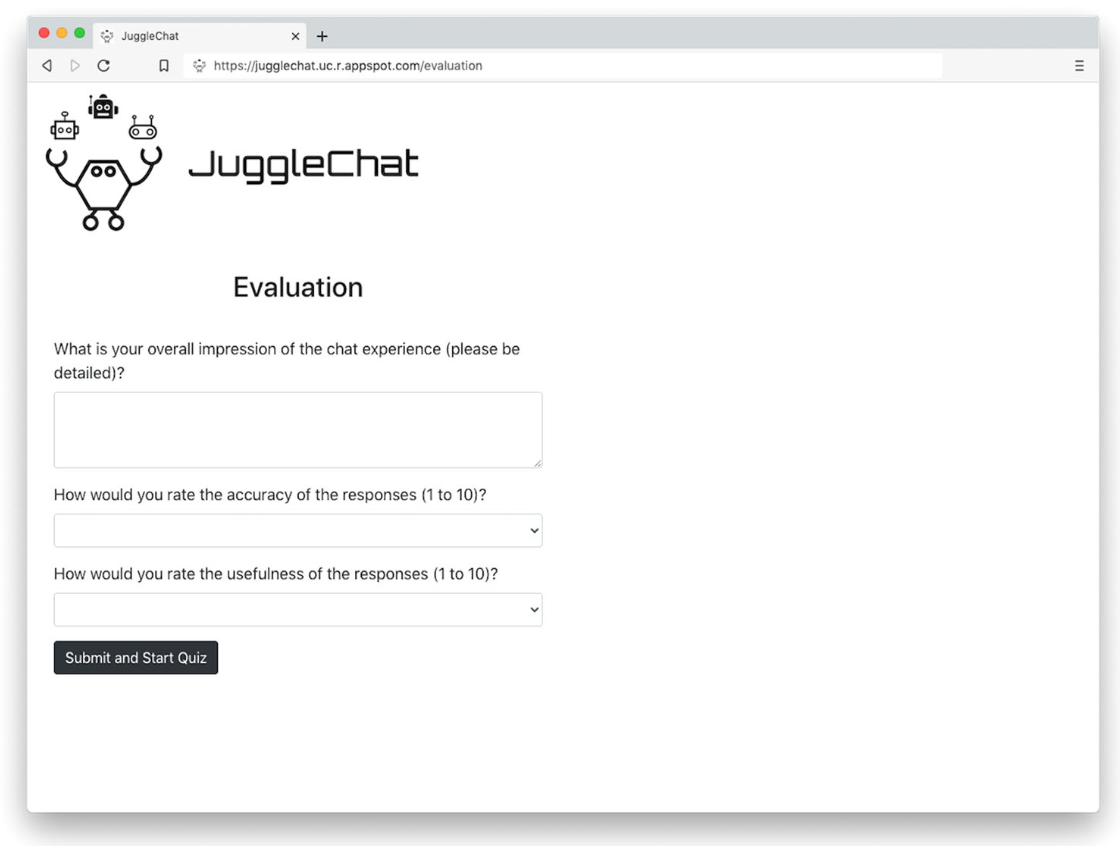
\includegraphics[width=16cm]{figuras/evaluation-briel.png}
    }{
		\Fonte{\citeonline{briel2021}.}
	}
\end{figure}

\begin{figure}[ht] 
   	\captionsetup{width=16cm}
	\Caption{\label{fig:quiz-briel} Questionário sobre o COVID-19}
	\UFCfig{}{
        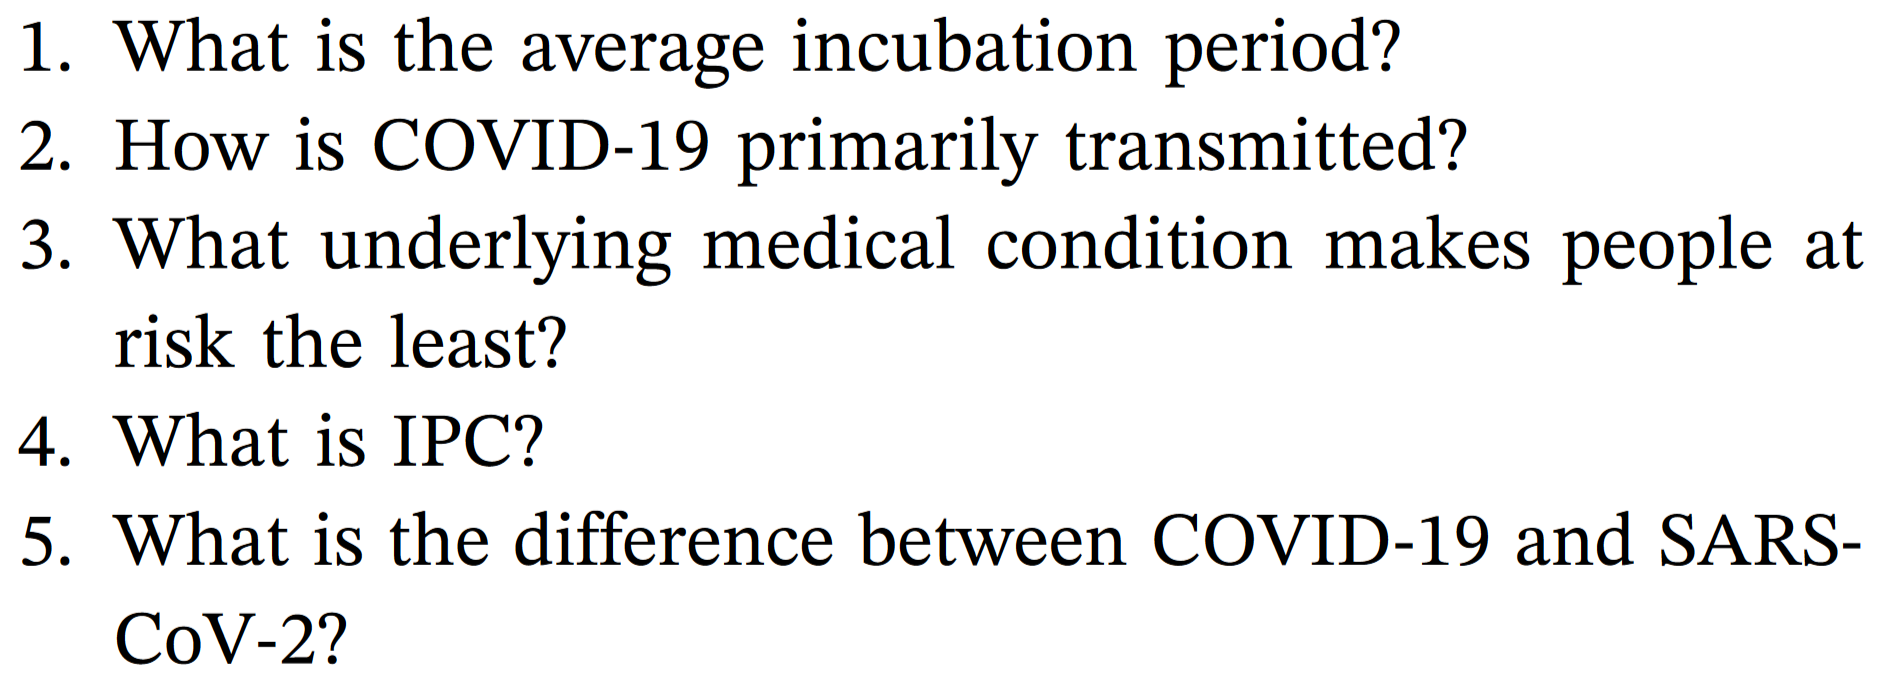
\includegraphics[width=16cm]{figuras/quiz-briel.png}
    }{
		\Fonte{\citeonline{briel2021}.}
	}
\end{figure}

Os resultados desse artigo mostraram que os participantes tiveram uma maior adesão ao chatbot baseado em respostas longas, ao passo que o chatbot baseado em respostas curtas foi avaliado como menos preciso e de menor utilidade. Por fim, o autor pontua que, diante de outros cenários de aprendizagem, essa preferência sobre o estilo do chatbot pode mudar. Assim, ele enfatiza a capacidade de adaptação do JuggleChat, devido a ele conseguir fornecer várias funcionalidades para atender às necessidades dos estudantes.